\chapter{Chapter One}
\section{Introduction}
Weather radar is an invaluable tool for nowcasting severe weather. In Canada, lake-effect snows are a
severe weather event which have adverse impacts on a large
sector of the population. While the current Canadian C-Band radar systems have been proven in this
regard, there is some uncertainty with how the specifications of the new S-Band systems will translate to lake-effect snow forecasting. While no prototype
system is available to test in the Great Lakes area, the next best stand-in to compare with are the current
S-Band
radars in the United States. King City radar (CWKR) has been compared with the Buffalo, NY radar (KBUF)
previously by \cite{Boodoo2015}, but this case was for deep, warm-season convection. Furthermore, C-Band radars have been compared with S-Band radars before
in other locales, e.g \citep{Abon2014,
WMO2008}, however polarimetric variables were not numerically compared on a large-scale. Our experimental setup is unique in that the radars are not co
located, in contrast with other research centers such as the University of Alabama
Huntsville, where a research C-Band radar is several kilometer away from a WSR-88D
\citep{Petersen2007}. With Lake Ontario in between CWKR and KBUF, this creates the opportunity to analyze a vast amount of incident sample volumes from lake
effect snow events. The one downfall is the addition of uncertainty stemming from differing elevation angles and beamwidths of the radars. In order to
accurately compare the two
radars, the data are objectively analyzed. Radar data objective analysis is most prominently used to
create mosaics of multiple radars for projects such as the National Severe Storm Laboratory's Multi-Radar Multi
Sensor in the U.S. \citep{Zhang2016}. It is also used extensively for research purposes, including studying
snow squalls \citep{Mulholland2017}.  The goal of this study is to investigate the differences in quality of radar observations between a C-Band and S
Band radar, for the purposes of
nowcasting lake-effect snow  Another goal is to directly compare polarimetric variables,
which has not been done in this manner before, and
identify any biases. It is important to remove biases as no amount of spatial or temporal smoothing will
remove them. With bias-adjusted values from two independent sources, a high-confidence conclusion can
be made on the types of hydrometeors present in the common sampling volumes. Although polarimetric radar has matured within the research community, operational deployment has been a much
slower process. Many studies have been undertaken in regards to quantitative precipitation estimation
using polarimetric variables for rainfall, but studies involving snow have been much more limited. Findings here
should increase confidence in comparing polarimetric at two different wavelengths, and demonstrate
the information rich nature of these variables. 
\section{Background}
First, it is important to provide some background on the weather radar moments that are presented in this study, from both single and dual polarized signals.
The convention for representing these moments symbolically hereafter is lower-case subscript for linear units and upper-case subscript for logarithmic units,
i.e. $Z_{DR}$ is logarithmic while $Z_{dr}$ is linear.
\subsection{Radar Locations}
In Canada, there is one active C-Band weather radar with dual-pol capabilities. It is located north of Toronto, in King City, while the rest of the network
is
currently undergoing an upgrade to polarimetric S-Band. Its neighbor to the south, KBUF, was upgraded to dual-pol in 2012 as part of a network wide upgrade.
The terms C-Band and S-Band are in reference to the frequency band in which a radar operates, thereby determining the wavelength they transmit. 
\begin{figure}[h]
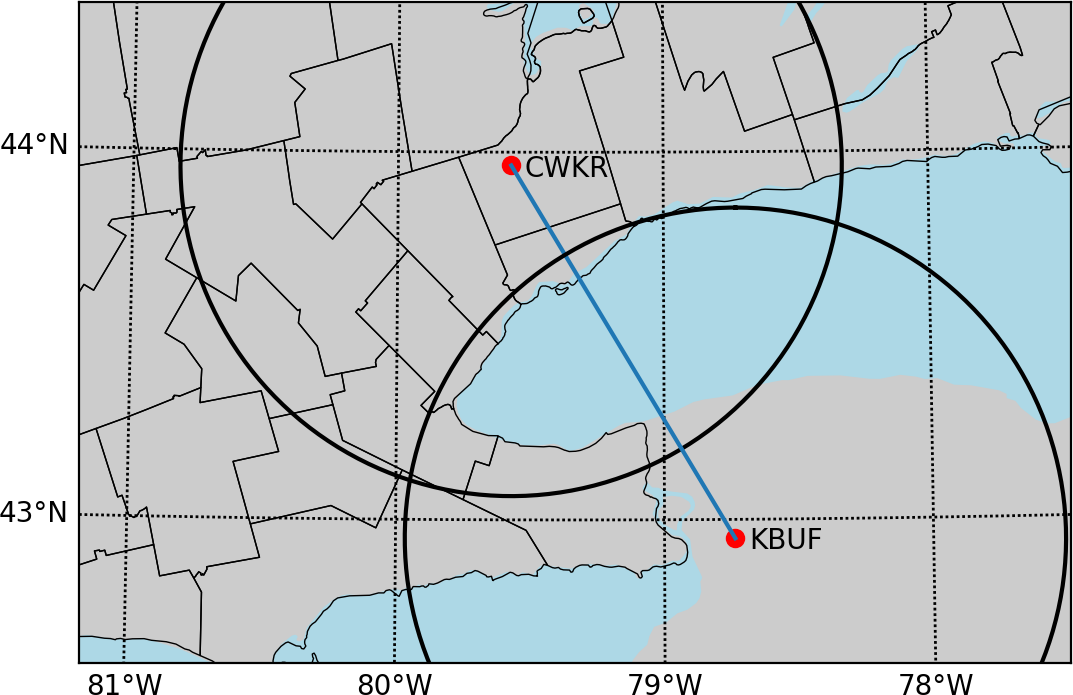
\includegraphics[width=\textwidth]{map}
\caption{The location of the NWS Buffalo Radar (KBUF) and King City Radar (CWKR) are shown as red dots, with a 100 km range ring around each. The distance
between the two, drawn as a blue line, is 131.5 km.} 
\label{map}
\end{figure}
Figure \ref{map} shows the geographic location of the radar sites in comparison with each other.
\subsection{Equivalent Reflectivity Factor ($Z_{h}$)}
The foremost moment derived from radar is the reflectivity factor ($Z_{h}$), where the
subscript denotes its derivation from the horizontally polarized signal. This variable
measures the number density $N(D)$ of hydrometeors of diameter $D$ per unit volume, as
presented in Equation \ref{eq:ref_factor}. Due to uncertainties about what type of
target is actually doing the scattering, it is typically represented as the equivalent
reflectivity factor $Z_{eh}$, where $Z_{h}$ = $Z_{eh}$ if the targets are made of liquid 
water and are comparatively small to the wavelength \citep{Fabry2015}. The two variables are 
essentially interchangeable, but the nomenclature \textit{equivalent} reflectivity factor will be used in this
study to acknowledge the presence of non-ideal targets, e.g. ice crystals/snow.
\begin{equation}\label{eq:ref_factor}
Z_{eh} \approx Z_{h} = \int_0^{\infty} N(D)D^6dD \ (mm^6/m^3)
\end{equation}
\subsection{Differential Reflectivity ($Z_{dr}$)}
Radars equipped with dual-pol capabilities are still an emerging technology, in terms of operational meteorological applications. These
types of radar systems are capable of transmitting and receiving two orthogonally polarized electromagnetic waves in order to deduce more information about
the microphysical structure of hydrometeors. One of the main variables this allows them to produce is $Z_{DR}$, \hl{defined as the logarithmic ratio of the 
horizontal channel reflectivity ($Z_h$) to the vertical channel reflectivity ($Z_{v}$)}. This can be simplified as the difference between the two, using the
logarithmic quotient rule. Equation \ref{eq:zdr} demonstrates this concept.
\begin{equation}\label{eq:zdr}
\mathcolorbox{yellow}{Z_{DR}} = 10 * \log_{10}(\frac{Z_h}{Z_v}) = Z_H - Z_V
\end{equation}
\subsubsection{Interpretations of $Z_{DR}$ in Snow}
In snowfall, $Z_{DR}$ can be a powerful tool for deducing the predominant crystal habit and type. Ranges of $Z_{DR}$ are typically given in the literature for characterizing hydrometeors, and vary due to their semi-empirical nature. The most widely cited synthesis paper by \citet{Straka2000} reports that dry aggregated snow at cold temperatures from $0 < Z_{DR} < 0.2$ dB, while pristine ice crystals and lightly aggregated crystals range from $0.4 < Z_{DR} < 3$ dB, both for a range of $Z_{eH}$ of $5 < Z_{eH} < 30$ dBZ. It should be noted that any riming of these particles would lead to a reduction in $Z_{DR}$, as they become more spherical \citet{Fabry2015} reports slightly different ranges in Figure \ref{zdr_chart}, and gives ranges for other targets beyond the scope of this study; hydrometeors that are sufficiently frozen are only considered in this study.
\begin{figure}[H]
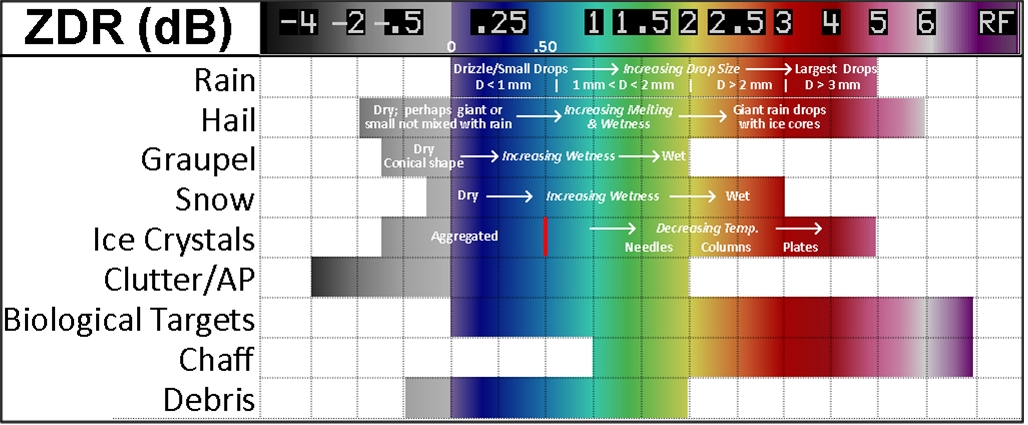
\includegraphics[width=\textwidth]{zdr_chart}
\caption{Chart of expected ranges of $Z_{DR}$ for a variety of targets. Taken from \citet{Fabry2015}.} 
\label{zdr_chart}
\end{figure}
\subsection{Co-polar Cross-Correlation Coefficient ($\rho_{hv}$)}
With the advent of Simultaneous Transmit and Receive (STAR) radar systems, which both radars used here have, it is possible to perform the zero time-lag
cross-correlation between the time series data obtained from horizontal and vertical channels. This is known as the Co-polar Cross-Correlation Coefficient
($\rho_{hv}$) in radar meteorology, and ranges from 0 to 1. Low values indicate pulse volumes containing heterogeneities, while a value of 1 indicates
matching, homogenous volumes. For an ensemble of scatters, Equation \ref{eq:backscatter} defines the back-scattering matrix used in the definition of
$\rho_{hv}$ in Equation \ref{eq:rhohv}, as defined by \citet{Ryzhkov2007b}. In essence, $S_{hh}$ ($S_{vv}$) is the backscattered signal produced by the horizontally (vertically) polarized signal, as measured in the horizontal (vertical) channel.
\begin{equation}\label{eq:backscatter}
\mathbf{S} = \begin{bmatrix}
             S_{hh}       & S_{hv} \\
             S_{hv}       & S_{vv} \\
             \end{bmatrix}
\end{equation}
\begin{equation}\label{eq:rhohv}
\rho_{hv} = \frac{\langle{S_{vv}{S_{hh}}^{*}\rangle}}{\sqrt{\langle{{S_{hh}}^{2}\rangle}\langle{{S_{vv}}^{2}\rangle}}}
\end{equation}
\subsubsection{Interpretations of $\rho_{hv}$ in Snow}
Contamination from clutter and other non-meteorological targets can be filtered by using a $\rho_{hv}$ threshold of 0.95, as suggested by \citet{Straka2000}.
Using this threshold can also be used to avoid Mie scatterers, which becomes a bigger problem at C-Band wavelengths \citep{Fabry2015}. Furthermore, this threshold reduces wavelength induced differences between the radar datasets.
 



